% !TeX program = xelatex
% !TeX encoding = UTF-8
% !TeX TXS-program:compile = txs:///xelatex | txs:///xelatex
\documentclass[aspectratio=169, table, 12pt]{beamer}

% Preamble bersama seluruh slide mata kuliah ini.
% Dipanggil dari slides/sessionXX/sessionXX.tex tepat sesudah baris
% \documentclass[aspectratio=169, table, 12pt]{beamer}
% Paket tambahan yang hanya dibutuhkan satu sesi ditulis di berkas sesi itu.

\usepackage{colortbl}
\usepackage{xcolor}
\usepackage{listings}
\usepackage{tabularx}
\usepackage{booktabs}
\usepackage{tikz}
\usepackage{pgfplots}
\usepackage{fontspec}
\usepackage[english,bahasai]{babel}
\pgfplotsset{compat=1.18}
\usetikzlibrary{arrows.meta, positioning, calc, fit, shapes.geometric,
  shapes.multipart, backgrounds, matrix, chains, trees}

\makeatletter
\def\input@path{{../theme/}}
\makeatother
\graphicspath{{../theme/}{../../figures/}}
% Stub symlink Windows memakai tema cadangan sampai aset institusi tersedia.
\IfFileExists{../theme/beamerthemePradita.sty}{%
  \usetheme{Pradita}
}{%
  \usetheme{Madrid}
  \setmainfont{TeX Gyre Heros}
  \setsansfont{TeX Gyre Heros}
  \setbeamertemplate{navigation symbols}{}
}

\definecolor{praditagreen}{RGB}{37, 113, 71}
\setbeamercolor{structure}{fg=praditagreen}
\setbeamercolor{palette primary}{bg=praditagreen,fg=white}
\setbeamercolor{palette secondary}{bg=praditagreen!80!black,fg=white}
\setbeamercolor{palette tertiary}{bg=praditagreen!60!black,fg=white}
\setbeamerfont{frametitle}{size=\large}
\setbeamertemplate{caption}[numbered]

% Ukuran header mengikuti teks agar judul panjang tidak menabrak logo.
\setbeamercolor{frametitle}{bg=white,fg=black}
\setbeamertemplate{frametitle}{%
  \begin{beamercolorbox}[wd=\paperwidth,sep=0.2cm]{frametitle}
    \begin{minipage}[c]{0.77\paperwidth}
      \raggedright\fontsize{16}{18}\selectfont\bfseries\insertframetitle
      \ifx\insertframesubtitle\empty\else
        \par\small\mdseries\insertframesubtitle
      \fi
    \end{minipage}\hfill
    \begin{minipage}[c]{0.15\paperwidth}
      \IfFileExists{../theme/classFiles/logo_universitas.png}{%
        
\includegraphics[width=\linewidth]{../theme/classFiles/logo_universitas.png}%
      }{}
    \end{minipage}
  \end{beamercolorbox}
}
\setbeamertemplate{footline}{%
  \ifnum\value{framenumber}>1
    \begin{beamercolorbox}[wd=\paperwidth,ht=0.35cm,dp=0.15cm,
      leftskip=0.3cm,rightskip=0.3cm]{palette primary}
      \footnotesize\bfseries\insertframenumber/\inserttotalframenumber
      \hfill IT40813
    \end{beamercolorbox}
  \fi
}
\DeclareRobustCommand{\berkas}[1]{\path{#1}}

% Tema membuat garis tabel berwarna putih. Dikembalikan agar tabel terbaca.
\arrayrulecolor{black}
\setlength{\arrayrulewidth}{0.5pt}

\lstdefinelanguage{yaml}{
  basicstyle=\ttfamily\scriptsize,
  keywordstyle=\color{blue}\bfseries,
  commentstyle=\color{gray}\itshape,
  stringstyle=\color{red},
  showstringspaces=false,
  breaklines=true,
  frame=lines,
  numbers=none,
  backgroundcolor=\color{lightgray!10},
  tabsize=2,
  morecomment=[l]{\#}
}

\lstdefinelanguage{json}{
  basicstyle=\ttfamily\scriptsize,
  stringstyle=\color{red},
  commentstyle=\color{gray},
  breaklines=true,
  showstringspaces=false,
  tabsize=2,
  numbers=none,
  frame=lines,
  backgroundcolor=\color{lightgray!10},
  string=[s]{"}{"}
}

\lstdefinelanguage{bash}{
  keywords={},
  basicstyle=\ttfamily\scriptsize,
  ndkeywords={docker, kubectl, helm, curl, git, terraform},
  ndkeywordstyle=\color{purple}\bfseries,
  sensitive=true,
  commentstyle=\color{gray},
  numbers=none,
  breaklines=true,
  frame=lines,
  backgroundcolor=\color{lightgray!10},
  tabsize=2,
  comment=[l]{\#},
  showstringspaces=false
}

\lstdefinelanguage{http}{
  keywords={GET, POST, PUT, PATCH, DELETE, HEAD, OPTIONS, HTTP},
  basicstyle=\ttfamily\scriptsize,
  keywordstyle=\color{blue}\bfseries,
  sensitive=true,
  numbers=none,
  breaklines=true,
  frame=lines,
  backgroundcolor=\color{lightgray!10},
  tabsize=2,
  showstringspaces=false
}

\subtitle{IT40813 · IT Governance, Risk \& Compliance}
\author{\textbf{Alfa Yohannis}}


% Sampul membatasi judul di panel putih tema rujukan Pradita.
\setbeamertemplate{title page}{%
  \begin{tikzpicture}[remember picture,overlay]
    \node[anchor=north west,inner sep=0pt,text width=8.8cm]
      at ([xshift=1cm,yshift=-3.15cm]current page.north west) {%
        {\small\insertsubtitle\par}\vspace{0.25cm}
        \resizebox{8.8cm}{!}{\begin{minipage}{12cm}
          \raggedright\color{praditagreen}\bfseries\inserttitle
        \end{minipage}}
      };
    \node[anchor=south west,inner sep=0pt]
      at ([xshift=1cm,yshift=1.65cm]current page.south west)
      {\small\insertdate};
    \node[anchor=west,inner sep=0pt,text=white]
      at ([xshift=0.8cm,yshift=0.75cm]current page.south west)
      {\small\insertauthor};
  \end{tikzpicture}
}


\title{\Huge Manajemen Risiko\\ \vspace{10pt} Enterprise dan Risiko TI}
\date{Pertemuan 05}

\begin{document}

\frame{\titlepage}

\begin{frame}
  \frametitle{Isi Pertemuan}
  \vspace{14pt}
  \begin{columns}[t]
    \column{0.5\textwidth}
    {\small\tableofcontents[sections={1-4}]}

    \column{0.5\textwidth}
    {\small\tableofcontents[sections={5-8}]}
  \end{columns}
\end{frame}

\begin{frame}{\hfill}
  \centering
  \Huge{\textbf{Register risiko 86 baris.\\Keputusan mana\\yang berubah?}}
\end{frame}

\section{Tujuan dan Konteks}

\begin{frame}{{\Large Tujuan Pembelajaran}}
  \vspace{10pt}
  \begin{itemize}
    \item Menerapkan proses ISO 31000 untuk mengidentifikasi, menganalisis, dan mengevaluasi risiko
          terkait TI.
    \item Merumuskan pernyataan \textit{risk appetite} yang dapat dipakai untuk mengambil keputusan.
    \item Membandingkan penilaian risiko kualitatif dan kuantitatif beserta keterbatasan
          masing-masing.
  \end{itemize}
\end{frame}

\begin{frame}{{\Large Masalah: Daftar Risiko Tidak Mengubah Keputusan}}
  \vspace{6pt}
  \small
  \begin{itemize}
    \item Misalkan register Medikara berisi 86 baris dan dibuka dua kali setahun menjelang audit.
    \item Kontrak vendor Medikara+ diperpanjang, tetapi baris tentang akun vendor tidak dibuka.
    \item Fakta kasus: kebocoran data skala kecil lewat vendor pada 2025 dan kontrol akses yang lemah.
    \item Tujuan, skenario, bukti kontrol, dan batas keputusan harus terhubung.
    \item Detail dan angka tambahan pada contoh adalah pengandaian. Luaran masuk tonggak C2.
  \end{itemize}
\end{frame}

\begin{frame}{{\Large Diagram Konsep Bab 5}}
  \centering
  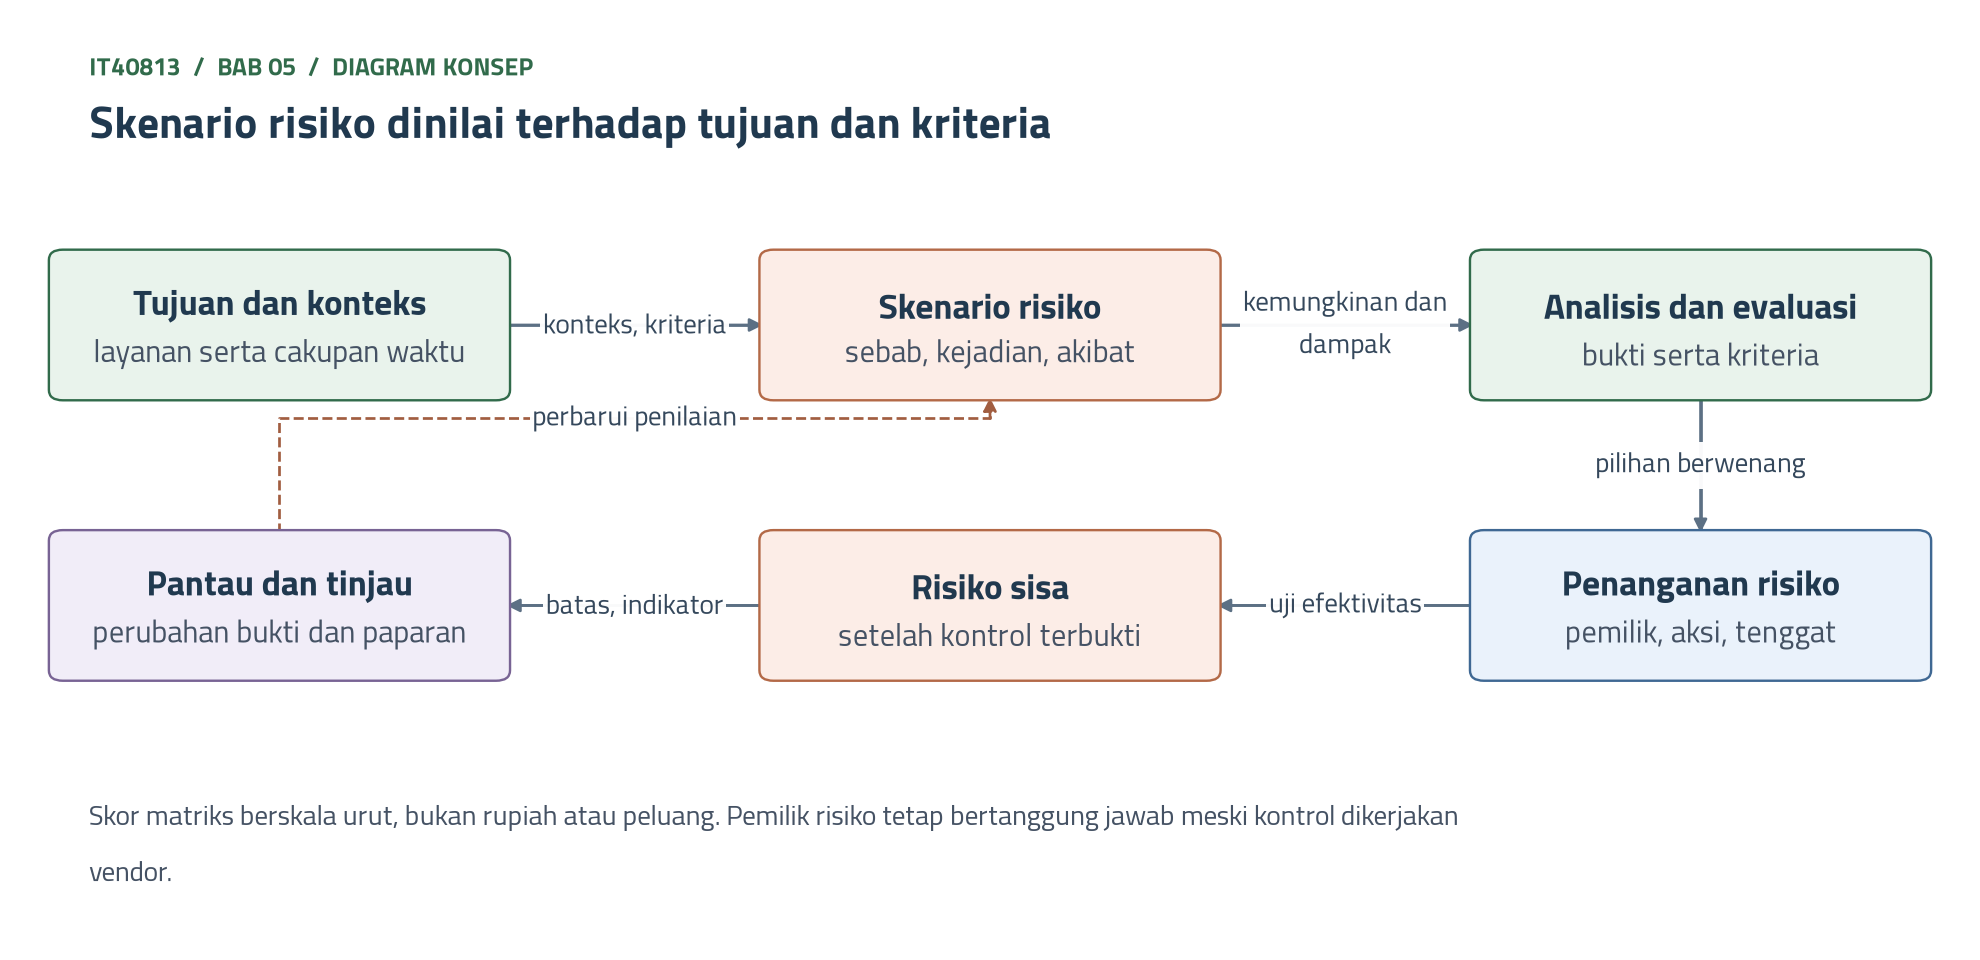
\includegraphics[width=0.96\textwidth,height=0.77\textheight,keepaspectratio]{../../figures/ch05-diagram-konsep.png}
  \label{fig:session05-ilustrasi-bab}
\end{frame}

\section{Risiko dan Tujuan}

\begin{frame}{{\Large Risiko Berawal dari Tujuan}}
  \vspace{6pt}
  \small
  \begin{itemize}
    \item ISO 31000:2018: risiko adalah efek ketidakpastian terhadap tujuan.
    \item Daftar ancaman belum menjadi penilaian risiko.
    \item ERM menghubungkan pilihan strategi dengan risiko portofolio, bukan sekadar mengumpulkan
          masalah departemen.
    \item Analogi ambulans: hujan menjadi risiko bila jalan tergenang dan pasien terlambat ditolong.
    \item Sekitar 1,2 juta kunjungan per tahun berarti sekitar 3.288 per hari. Misalkan layanan 12 jam:
          gangguan pendaftaran 3 jam menyentuh sekitar 822 kunjungan.
    \item Misalkan 216 berkas klinik per tahun. Satu klinik mengubah format: 1 dari 18 berkas bulanan,
          sekitar 5,6 persen, salah terbaca.
  \end{itemize}
\end{frame}

\begin{frame}{{\Large Tujuan, Risiko, dan Keputusan}}
  \vspace{4pt}
  \footnotesize
  \begin{tabularx}{\textwidth}{|>{\raggedright\arraybackslash}p{0.22\textwidth}|>{\raggedright\arraybackslash}X|>{\raggedright\arraybackslash}X|}
    \hline
    \textbf{Tujuan} & \textbf{Skenario} & \textbf{Keputusan} \\ \hline
    Kerahasiaan data & R-01: akses vendor berlebihan menyebabkan pengungkapan data pasien & Batasi
    akses dan tinjau AC-01 \\ \hline
    Kelangsungan pendaftaran & R-03: integrasi BPJS Kesehatan terhenti ketika pasien datang &
    Siapkan antrean pengganti \\ \hline
    Laporan konsisten & R-04: versi spreadsheet berbeda & Tetapkan validasi dan pemilik definisi \\
    \hline
    Keselamatan pasien & R-11: riwayat alergi tidak terbaca lintas rumah sakit & Libatkan pimpinan
    klinis dan perbaiki pertukaran data \\ \hline
  \end{tabularx}

  \vspace{6pt}
  \small Risiko berbeda dari temuan. 6 dari 30 akun sampel adalah temuan yang perlu ditutup.
  Kemungkinan akun itu dipakai mengakses data adalah risiko yang perlu diputuskan.
\end{frame}

\begin{frame}{{\Large Lima Komponen COSO ERM}}
  \vspace{4pt}
  \footnotesize
  \begin{tabularx}{\textwidth}{|>{\raggedright\arraybackslash}p{0.36\textwidth}|>{\raggedright\arraybackslash}X|}
    \hline
    \textbf{Komponen} & \textbf{Contoh penerapan pada Medikara} \\ \hline
    Tata kelola dan budaya & Komite 9 anggota, kuorum 6, pemilik risiko wajib hadir \\ \hline
    Strategi dan penetapan sasaran & ``Satu Pasien, Satu Rekam Medis'' menurunkan \textit{risk
    appetite} \\ \hline
    Kinerja & Register 12 skenario dinilai, diprioritaskan, dan diberi keputusan \\ \hline
    Tinjauan dan revisi & Insiden 2025 dan temuan audit memicu penilaian ulang R-01 \\ \hline
    Informasi, komunikasi, dan pelaporan & Indikator dan laporan satu halaman pada Bab 13 \\ \hline
  \end{tabularx}

  \vspace{6pt}
  \small Lima komponen dan 20 prinsip, bukan tahap berurutan. Contoh merupakan pengandaian.
\end{frame}

\begin{frame}{{\Large Risiko TI di dalam Risiko Enterprise}}
  \vspace{4pt}
  \footnotesize
  \begin{tabularx}{\textwidth}{|>{\raggedright\arraybackslash}p{0.17\textwidth}|>{\raggedright\arraybackslash}X|>{\raggedright\arraybackslash}X|>{\raggedright\arraybackslash}X|}
    \hline
    \textbf{Tingkat} & \textbf{Pertanyaan} & \textbf{Pemeran} & \textbf{Keluaran} \\ \hline
    Organisasi & Risiko mana yang menyentuh strategi? & Direksi, komite, kepala risiko &
    \textit{Risk appetite}, profil risiko \\ \hline
    Proses misi dan bisnis & Layanan mana yang terdampak? & Pemilik Medikara+, kepala pendaftaran &
    \textit{Risk tolerance}, register layanan \\ \hline
    Sistem informasi & Kontrol mana yang berjalan? & Kepala operasi TI, pengelola SIMRS & Bukti
    kontrol, register sistem \\ \hline
  \end{tabularx}

  \vspace{6pt}
  \small Misalkan 5 rumah sakit mengirim 14 baris per rumah sakit, atau 70 baris. Delapan baris
  tentang hak akses SIMRS lokal digabung menjadi R-02. Tiga tingkat mengikuti NIST SP 800-39.
\end{frame}

\section{Proses ISO 31000}

\begin{frame}{{\Large Prinsip, Kerangka, dan Proses}}
  \vspace{6pt}
  \small
  \begin{itemize}
    \item ISO 31000:2018 memberi panduan, bukan persyaratan sertifikasi organisasi.
    \item Delapan prinsip: terintegrasi, terstruktur dan menyeluruh, disesuaikan, inklusif, dinamis,
          informasi terbaik, faktor manusia dan budaya, terus diperbaiki.
    \item Cakupan, konteks, dan kriteria ditetapkan sebelum penilaian.
    \item Analogi kendaraan: ban tipis adalah temuan awal, peluang tergelincir adalah analisis,
          batas aman adalah evaluasi, mengganti ban adalah penanganan.
    \item Misalkan cakupan Medikara+ 12 bulan: 336.000 janji temu dan 120 akun vendor.
  \end{itemize}
\end{frame}

\begin{frame}{{\Large Proses dari Konteks hingga Keputusan}}
  \centering
  \vspace{6pt}
  \resizebox{\textwidth}{!}{\begin{tikzpicture}[
  font=\scriptsize,
  tahap/.style={draw, rounded corners, align=center, text width=1.75cm,
    minimum height=1.25cm, fill=blue!8},
  pita/.style={draw, rounded corners, align=center, text width=10.5cm,
    minimum height=0.55cm, fill=praditagreen!15},
  panah/.style={-{Stealth[length=2mm]}, thick}]
  \node[pita] (komunikasi) at (4.5,1.5)
    {Komunikasi dan konsultasi: pemilik layanan, klinis, hukum, keuangan, dan TI};
  \node[tahap] (konteks) at (0,0) {Cakupan, konteks, dan kriteria};
  \node[tahap, fill=orange!12] (identifikasi) at (2.25,0) {Identifikasi\\skenario};
  \node[tahap, fill=orange!12] (analisis) at (4.5,0) {Analisis\\kemungkinan\\dan dampak};
  \node[tahap, fill=orange!12] (evaluasi) at (6.75,0) {Evaluasi\\terhadap\\kriteria};
  \node[tahap, fill=green!10] (penanganan) at (9,0) {Penanganan\\dan\\risiko sisa};
  \node[pita] (pantau) at (4.5,-1.5)
    {Pantau dan tinjau: perubahan bukti, paparan, dan efektivitas kontrol};
  \node[pita] (catat) at (4.5,-2.2)
    {Pencatatan dan pelaporan: \textit{risk register} dan bahan keputusan};
  \draw[panah] (konteks) -- (identifikasi);
  \draw[panah] (identifikasi) -- (analisis);
  \draw[panah] (analisis) -- (evaluasi);
  \draw[panah] (evaluasi) -- (penanganan);
  \draw[thick, decorate] (identifikasi.north west) ++(0,0.08) -- ++(0,0.1)
    -| ([yshift=0.08cm]evaluasi.north east);
  \node[fill=white, inner sep=1pt] at (4.5,0.84) {{\tiny\mdseries penilaian risiko}};
  \draw[panah] (penanganan.south) -- (penanganan.south |- pantau.north);
  \draw[panah, dashed] (pantau.north -| identifikasi) -- (identifikasi.south)
    node[midway, right] {{\tiny\mdseries perbarui penilaian}};
\end{tikzpicture}
}

  \vspace{4pt}
  {\footnotesize Ringkasan pembelajaran, bukan reproduksi gambar standar.}
\end{frame}

\begin{frame}{{\Large Kriteria Ditetapkan sebelum Skor}}
  \vspace{2pt}
  \footnotesize
  \begin{tabularx}{\textwidth}{|>{\raggedright\arraybackslash}p{0.07\textwidth}|>{\raggedright\arraybackslash}p{0.28\textwidth}|>{\raggedright\arraybackslash}p{0.3\textwidth}|>{\raggedright\arraybackslash}X|}
    \hline
    \textbf{Nilai} & \textbf{Kemungkinan (12 bulan)} & \textbf{Dampak finansial} & \textbf{Dampak
    layanan} \\ \hline
    1 & Kurang dari 5 persen & Di bawah Rp10 juta & Pulih dalam unit \\ \hline
    2 & 5 sampai kurang dari 15 persen & Rp10 juta sampai kurang dari Rp50 juta & Gangguan lokal \\ \hline
    3 & 15 sampai kurang dari 40 persen & Rp50 juta sampai kurang dari Rp200 juta & Layanan penting
    tertunda \\ \hline
    4 & 40 sampai kurang dari 70 persen & Rp200 juta sampai kurang dari Rp1 miliar & Gangguan lintas
    lokasi \\ \hline
    5 & 70 persen atau lebih & Rp1 miliar atau lebih & Layanan utama berhenti \\ \hline
  \end{tabularx}

  \vspace{5pt}
  \small Contoh, bukan skala baku. Skala tidak diubah setelah melihat hasil. Keselamatan dan
  kepatuhan dinilai pada kolom terpisah.
\end{frame}

\begin{frame}{{\Large Mulai dari Peristiwa atau Aset?}}
  \vspace{2pt}
  \footnotesize
  \begin{tabularx}{\textwidth}{|>{\raggedright\arraybackslash}p{0.17\textwidth}|>{\raggedright\arraybackslash}X|>{\raggedright\arraybackslash}X|}
    \hline
    \textbf{Unsur} & \textbf{Berbasis peristiwa} & \textbf{Berbasis aset} \\ \hline
    Titik awal & Kejadian dan akibatnya pada tujuan & Data, sistem, dan ketergantungan \\ \hline
    Contoh & Insiden vendor 2025, gangguan BPJS Kesehatan & Rekam medis, SIMRS, Medikara+ \\ \hline
    Mudah terlewat & Aset yang belum pernah terkena masalah & Kejadian lintas aset, misalnya satu
    subpenyedia \\ \hline
  \end{tabularx}

  \vspace{6pt}
  \small
  \begin{itemize}
    \item Misalkan 9 skenario dari peristiwa, 8 dari aset, 5 sama: 12 skenario unik.
    \item NIST SP 800-30 Rev. 1: titik awal dapat membuat risiko terlewat. Sudut pandang kedua
          meningkatkan ketelitian.
  \end{itemize}
\end{frame}

\section{Risk Appetite dan Batas}

\begin{frame}{{\Large Risk Appetite, Risk Tolerance, Kapasitas}}
  \vspace{6pt}
  \small
  \begin{itemize}
    \item \textit{Risk appetite}: arah risiko yang bersedia diambil, dari pimpinan tertinggi.
    \item \textit{Risk tolerance}: batas operasional yang selalu lebih spesifik.
    \item Kapasitas risiko: batas yang mampu ditanggung.
    \item Mampu membayar tidak berarti boleh melanggar kewajiban hukum atau mengabaikan keselamatan.
    \item Analogi: anggaran perjalanan, batas penyimpangan, dan dana kebutuhan pokok keluarga.
  \end{itemize}
\end{frame}

\begin{frame}{{\Large Empat Lapis Batas untuk R-01}}
  \centering
  \vspace{2pt}
  \resizebox{\textwidth}{!}{\begin{tikzpicture}[
  font=\scriptsize,
  execute at begin node={\hyphenpenalty=10000\exhyphenpenalty=10000},
  isi/.style={anchor=north west, align=left, text width=9.6cm, inner sep=2pt}]
  \draw[rounded corners, fill=praditagreen!15] (0,0) rectangle (11.4,5.3);
  \node[isi, text width=11cm] at (0.15,5.22)
    {\textbf{Kapasitas risiko:} batas yang mampu ditanggung, misalkan Rp5 miliar per tahun.};
  \draw[rounded corners, fill=orange!12] (0.4,0.45) rectangle (11,4.75);
  \node[isi, text width=10.2cm] at (0.55,4.67)
    {\textbf{\textit{Risk appetite}:} arah yang disahkan direksi. Rendah untuk akses tidak sah
    pada data pasien. Peluang kerugian Rp1,5 miliar atau lebih paling tinggi 2 persen per
    tahun.};
  \draw[rounded corners, fill=blue!8] (0.8,0.65) rectangle (10.6,3.6);
  \node[isi, text width=9.4cm] at (0.95,3.52)
    {\textbf{\textit{Risk tolerance}:} batas operasional. Nol akun vendor aktif tanpa pemilik
    dan masa berlaku. Pencabutan paling lambat 1 hari kerja setelah penugasan berakhir.};
  \draw[rounded corners, fill=green!10] (1.2,0.85) rectangle (10.2,2.4);
  \node[isi, text width=8.6cm] at (1.35,2.32)
    {\textbf{KRI dan bukti:} jumlah akun tanpa pemilik, akun melewati masa berlaku, dan hasil
    AC-01. Nilai di luar batas memicu pembekuan akun dan keputusan pemilik risiko.};
  \node[anchor=south, align=center] at (5.7,0.06)
    {{\tiny\mdseries Keselamatan pasien dan kewajiban hukum dinilai terpisah, bukan ditukar
    dengan rupiah.}};
\end{tikzpicture}
}
\end{frame}

\begin{frame}{{\Large Usulan Batas Keputusan Medikara (Misalkan)}}
  \vspace{2pt}
  \scriptsize
  \begin{tabularx}{\textwidth}{|>{\raggedright\arraybackslash}p{0.14\textwidth}|>{\raggedright\arraybackslash}X|>{\raggedright\arraybackslash}X|>{\raggedright\arraybackslash}p{0.23\textwidth}|}
    \hline
    \textbf{Kategori} & \textbf{Arah} & \textbf{Ukuran} & \textbf{Pemicu tindakan} \\ \hline
    Keselamatan pasien & Tidak menukar risiko cedera berat dengan kecepatan atau biaya & Risiko cedera
    berat ditinjau dalam 1 hari kerja & Libatkan pimpinan klinis segera \\ \hline
    Kerahasiaan & Rendah untuk akses tidak sah pada data pasien & Nol akun vendor aktif tanpa pemilik
    dan masa berlaku & Bekukan akun yang tidak sesuai \\ \hline
    Kelangsungan & Menerima gangguan singkat bila prosedur pengganti berjalan & Pendaftaran terganggu
    paling lama 2 jam per bulan & Pemilik layanan menyiapkan perbaikan \\ \hline
    Kepatuhan & Rendah untuk kewajiban hukum yang terlewat & K-01 sampai K-16 memiliki pemilik; nol
    baris lewat tenggat & Catat penyimpangan dan tindakan \\ \hline
    Finansial & Membatasi kerugian besar & Peluang kerugian Rp1,5 miliar atau lebih paling tinggi 2
    persen per tahun & Laporkan ke komite \\ \hline
  \end{tabularx}
\end{frame}

\begin{frame}{{\Large Menguji Pernyataan Risk Appetite}}
  \vspace{6pt}
  \small
  \begin{itemize}
    \item ``Tidak menoleransi kebocoran data'' belum memberi aturan kerja.
    \item Empat pertanyaan: menyebut yang diterima dan ditolak? ada ukuran? memicu tindakan dan
          menyebut pemilik? sejalan dengan kewajiban hukum?
    \item Contoh NIST, penyedia layanan kesehatan: \textit{risk appetite} rendah untuk kontrol akses
          yang tidak memadai; 100 persen aplikasi kritis wajib memakai MFA.
    \item Medikara: 1 dari 120 akun tanpa pemilik, sekitar 0,8 persen, tetap diblokir.
    \item Denda paling tinggi 2 persen dari Rp500 miliar, yaitu Rp10 miliar, melewati kapasitas
          pengandaian Rp5 miliar.
  \end{itemize}
\end{frame}

\begin{frame}{{\Large Kasus Medikara: Batas yang Disahkan Direksi}}
  \vspace{6pt}
  \small
  \begin{itemize}
    \item Misalkan komite membahas batas dengan 7 dari 9 anggota hadir, kuorum 6 terpenuhi.
    \item Vendor meminta 4 akun tetap aktif 10 hari setelah penugasan berakhir: 40 akun-hari.
    \item Pemilik Medikara+ menolak dan memberi pengecualian darurat 24 jam: 4 akun-hari, turun 90
          persen.
    \item Konsekuensi pertama: perbaikan vendor lebih lambat, tenggat bergeser 3 hari.
    \item Konsekuensi kedua: bahasan berpindah ke bukti pengecualian dan pihak yang menyetujui.
  \end{itemize}
\end{frame}

\section{Risk Register}

\begin{frame}{{\Large Register Menyimpan Alasan Keputusan}}
  \vspace{6pt}
  \small
  \begin{itemize}
    \item Satu baris: pengenal, tujuan, sebab, kejadian, akibat, pemilik, bukti, kontrol, penilaian,
          rencana.
    \item Pemilik risiko mengelola akibat. Pelaksana kontrol teknis dapat berbeda.
    \item Analogi buku piutang: jumlah, jatuh tempo, dan penagih membuat catatan berguna.
    \item AC-01: 6 dari 30 akun sampel dan 24 dari 120 akun, sama-sama 20 persen.
    \item Pengandaian Bab 4: daftar hanya 108 akun, 12 akun atau 10 persen luput.
  \end{itemize}
\end{frame}

\begin{frame}{{\Large Skenario R-01: Sebab, Kejadian, Akibat}}
  \centering
  \vspace{8pt}
  \resizebox{\textwidth}{!}{\begin{tikzpicture}[
  font=\scriptsize,
  execute at begin node={\hyphenpenalty=10000\exhyphenpenalty=10000},
  kotak/.style={draw, rounded corners, align=center, text width=1.95cm,
    minimum height=1.9cm, fill=blue!8},
  pita/.style={draw, rounded corners, align=center, minimum height=0.55cm},
  panah/.style={-{Stealth[length=2mm]}, thick}]
  \node[pita, text width=11.5cm, fill=praditagreen!15] (tujuan) at (4.9,1.55)
    {Tujuan: kerahasiaan data pasien. Pemilik risiko: pemilik Medikara+.
    Pelaksana kontrol: kepala operasi TI.};
  \node[kotak] (sebab) at (0,0)
    {\textbf{Sebab}\\akun vendor aktif setelah penugasan berakhir};
  \node[kotak, fill=green!10] (cegah) at (2.45,0)
    {\textbf{Kontrol pencegah}\\AC-01 dan pencabutan 1 hari kerja};
  \node[kotak, fill=orange!12] (kejadian) at (4.9,0)
    {\textbf{Kejadian}\\R-01: akses vendor menyimpang};
  \node[kotak, fill=green!10] (batas) at (7.35,0)
    {\textbf{Kontrol pembatas}\\pemantauan \textit{log} dan prosedur $3 \times 24$ jam};
  \node[kotak, fill=red!22] (akibat) at (9.8,0)
    {\textbf{Akibat}\\data pasien terungkap, biaya, dan sanksi};
  \node[pita, text width=5.55cm, fill=gray!35] (kiri) at (1.85,-1.45)
    {Bekerja sebelum kejadian: menurunkan kemungkinan};
  \node[pita, text width=5.55cm, fill=gray!35] (kanan) at (7.95,-1.45)
    {Bekerja sesudah kejadian: membatasi dampak};
  \draw[panah] (sebab) -- (cegah);
  \draw[panah] (cegah) -- (kejadian);
  \draw[panah] (kejadian) -- (batas);
  \draw[panah] (batas) -- (akibat);
\end{tikzpicture}
}
\end{frame}

\begin{frame}{{\Large Bagian Register Kondisi Saat Ini (Misalkan)}}
  \vspace{2pt}
  \scriptsize
  \begin{tabularx}{\textwidth}{|>{\raggedright\arraybackslash}p{0.2\textwidth}|>{\raggedright\arraybackslash}X|>{\raggedright\arraybackslash}p{0.13\textwidth}|>{\raggedright\arraybackslash}X|}
    \hline
    \textbf{ID dan pemilik} & \textbf{Skenario} & \textbf{Skor} & \textbf{Kontrol dan pemeriksaan} \\
    \hline
    R-01, pemilik Medikara+ & Akses vendor berlebihan, data pasien terungkap & $3 \times 4 = 12$ & AC-01
    belum lengkap; cocokkan 120 akun \\ \hline
    R-02, pemilik SIMRS & Hak akses lokal berbeda antar-rumah sakit & $3 \times 4 = 12$ & Persetujuan
    lokal; periksa pencabutan \\ \hline
    R-03, kepala pendaftaran & Integrasi BPJS Kesehatan terhenti & $3 \times 3 = 9$ & Antrean manual
    belum dilatih \\ \hline
    R-04, kepala pelaporan & Versi spreadsheet berbeda & $4 \times 3 = 12$ & Rekonsiliasi bulanan \\
    \hline
    R-05, pemilik layanan & Cadangan belum diuji, pemulihan gagal & $2 \times 5 = 10$ & Cadangan malam;
    uji pemulihan \\ \hline
    R-11, direktur pelayanan & Riwayat alergi tidak terbaca, kesalahan obat & $3 \times 4 = 12$ &
    Keselamatan; tinjauan klinis \\ \hline
  \end{tabularx}
\end{frame}

\begin{frame}{{\Large Kasus Medikara: Dari 86 Baris ke 12 Skenario}}
  \vspace{6pt}
  \small
  \begin{itemize}
    \item 38 baris digabung, 21 baris dipindah ke daftar temuan, 15 baris di luar cakupan: tersisa 12.
    \item Satu pemilik untuk tiap skenario. Komite dapat membacanya dalam rapat 2 jam.
    \item Pengenal lama tetap terlacak untuk audit.
    \item Baris R-01 menulis ``AC-01 sebagian'', bukan ``AC-01 ada''.
    \item Data latihan Bab 1 (1.240 rekam, Rp23,7 juta) bukan hasil investigasi: register menulis
          ``belum ada bukti''. Angka lain adalah asumsi pembelajaran.
  \end{itemize}
\end{frame}

\section{Matriks dan Kuantifikasi}

\begin{frame}{{\Large Matriks Risiko: 12 Skenario Contoh}}
  \centering
  \vspace{2pt}
  \resizebox{\textwidth}{!}{\begin{tikzpicture}[
  font=\scriptsize,
  execute at begin node={\hyphenpenalty=10000\exhyphenpenalty=10000},
  sel/.style={draw, minimum width=1.6cm, minimum height=0.95cm, inner sep=0pt},
  legenda/.style={draw, minimum width=0.45cm, minimum height=0.32cm, inner sep=0pt},
  kode/.style={align=center, font=\tiny}]
  \foreach \kemungkinan in {1,...,5} {
    \foreach \dampak in {1,...,5} {
      \pgfmathtruncatemacro{\skor}{\kemungkinan*\dampak}
      \ifnum\skor<5 \def\warna{green!10}\else
        \ifnum\skor<10 \def\warna{blue!8}\else
          \ifnum\skor<15 \def\warna{orange!12}\else
            \def\warna{red!22}\fi\fi\fi
      \node[sel, fill=\warna] at (\kemungkinan*1.6, \dampak*0.95) {};
      \node[anchor=north west, inner sep=1.5pt, font=\tiny\bfseries]
        at (\kemungkinan*1.6-0.8, \dampak*0.95+0.475) {\skor};
      \node[font=\scriptsize] at (\kemungkinan*1.6, 0.25) {\kemungkinan};
      \node[font=\scriptsize] at (0.58, \dampak*0.95) {\dampak};
    }
  }
  \node at (4.8,-0.1) {Kemungkinan (skala urut, 12 bulan)};
  \node[rotate=90] at (0.22,2.85) {Dampak (skala urut)};
  \node[kode] at (4.8,3.72) {R-01, R-02\\R-11};
  \node[kode] at (6.4,2.77) {R-04};
  \node[kode] at (3.2,4.67) {R-05};
  \node[kode] at (4.8,2.77) {R-03, R-06\\R-07, R-09};
  \node[kode] at (3.2,3.72) {R-08, R-10\\R-12};
  \node[legenda, fill=green!10] at (9.1,4.8) {};
  \node[anchor=west] at (9.35,4.8) {1 sampai 4, rendah};
  \node[legenda, fill=blue!8] at (9.1,4.3) {};
  \node[anchor=west] at (9.35,4.3) {5 sampai 9, sedang};
  \node[legenda, fill=orange!12] at (9.1,3.8) {};
  \node[anchor=west] at (9.35,3.8) {10 sampai 14, tinggi};
  \node[legenda, fill=red!22] at (9.1,3.3) {};
  \node[anchor=west] at (9.35,3.3) {15 sampai 25, kritis};
  \node[anchor=north west, align=left, text width=2.75cm] at (8.85,2.8)
    {{\tiny\mdseries R-11 berkaitan dengan keselamatan pasien. Skornya sama dengan R-01, R-02,
    dan R-04, tetapi jalur eskalasinya berbeda.}};
\end{tikzpicture}
}
\end{frame}

\begin{frame}{{\Large Skor Sama, Keputusan Berbeda}}
  \vspace{2pt}
  \footnotesize
  \begin{tabularx}{\textwidth}{|>{\raggedright\arraybackslash}X|>{\raggedright\arraybackslash}p{0.12\textwidth}|>{\raggedright\arraybackslash}p{0.17\textwidth}|>{\raggedright\arraybackslash}p{0.15\textwidth}|>{\raggedright\arraybackslash}p{0.16\textwidth}|}
    \hline
    \textbf{Skenario} & \textbf{Peluang} & \textbf{Kerugian} & \textbf{Skor} & \textbf{Harapan} \\ \hline
    R-01 akses vendor & 0,2 & Rp500 juta & $3 \times 4 = 12$ & Rp100 juta \\ \hline
    R-04 laporan spreadsheet & 0,5 & Rp60 juta & $4 \times 3 = 12$ & Rp30 juta \\ \hline
    R-05 pemulihan gagal & 0,1 & Rp2 miliar & $2 \times 5 = 10$ & Rp200 juta \\ \hline
  \end{tabularx}

  \vspace{6pt}
  \small
  \begin{itemize}
    \item Skor berskala urut, bukan rupiah atau peluang. Dampak 4 bukan dua kali dampak 2.
    \item R-11 dan R-04 sama-sama 12, tetapi hanya R-11 menyangkut keselamatan pasien.
    \item Analogi: peringkat kedua tidak berlari dua kali lebih cepat daripada peringkat keempat.
  \end{itemize}
\end{frame}

\begin{frame}{{\Large Kelemahan Matriks dan Cara Memakainya}}
  \vspace{6pt}
  \small
  \begin{itemize}
    \item Cox (2008): resolusi buruk, peringkat dapat terbalik, alokasi sumber daya tidak efektif,
          masukan dan keluaran perlu tafsir subjektif.
    \item Thomas dan rekan (2014): struktur matriks menghasilkan keputusan yang arbitrer.
    \item Penafsiran bab ini: matriks tetap berguna sebagai penyaring dan bahan diskusi.
    \item Definisikan skala lebih dahulu; pisahkan keselamatan dan kepatuhan.
    \item Skor sama bukan anggaran sama; hitung lebih lanjut sebelum membeli kontrol.
  \end{itemize}
\end{frame}

\begin{frame}{{\Large Kualitatif, Semi-kuantitatif, Kuantitatif}}
  \vspace{2pt}
  \footnotesize
  \begin{tabularx}{\textwidth}{|>{\raggedright\arraybackslash}p{0.17\textwidth}|>{\raggedright\arraybackslash}X|>{\raggedright\arraybackslash}X|>{\raggedright\arraybackslash}X|}
    \hline
    \textbf{Pendekatan} & \textbf{Bentuk nilai} & \textbf{Kekuatan} & \textbf{Keterbatasan} \\ \hline
    Kualitatif & Rendah, sedang, tinggi & Mudah disampaikan & Rentang kecil; hasil antarahli berbeda \\
    \hline
    Semi-kuantitatif & Skala yang maknanya hanya berlaku dalam konteks itu & Perbandingan relatif &
    Penilaian subjektif dapat tersembunyi \\ \hline
    Kuantitatif & Angka yang maknanya terjaga di luar konteks & Mendukung analisis biaya dan manfaat &
    Asumsi perlu dijelaskan; biaya keahlian \\ \hline
  \end{tabularx}

  \vspace{6pt}
  \small Menurut NIST SP 800-30 Rev. 1. Matriks $5 \times 5$ termasuk semi-kuantitatif.
\end{frame}

\begin{frame}{{\Large Dua Pertanyaan: Seberapa Sering, Seberapa Besar}}
  \vspace{6pt}
  \small
  \begin{itemize}
    \item Misalkan peluang insiden vendor 0,2 per tahun dan kerugian bersyarat rata-rata Rp500 juta:
          harapan Rp100 juta per tahun.
    \item Harapan bukan kerugian tahunan. Sebagian besar tahun nol, tahun insiden jauh lebih besar.
    \item Sebaran per kejadian: Rp100 juta (0,5), Rp500 juta (0,3), Rp1,5 miliar (0,2).
    \item Tiga titik Rp100 juta, Rp400 juta, Rp1,5 miliar: rata-rata sederhana sekitar Rp667 juta,
          bobot empat sekitar Rp533 juta.
    \item Analogi cuaca: peluang hujan 30 persen bukan janji, tetapi tetap berguna untuk memutuskan.
  \end{itemize}
\end{frame}

\begin{frame}{{\Large Loss Exceedance Curve R-01 (Misalkan)}}
  \centering
  \vspace{2pt}
  \resizebox{!}{0.72\textheight}{\begin{tikzpicture}[font=\scriptsize]
  \begin{axis}[
    width=11cm,
    height=6cm,
    xmin=0,
    xmax=2000,
    ymin=0,
    ymax=25,
    xtick={100,500,1500},
    xticklabels={Rp100 juta, Rp500 juta, {Rp1,5 miliar}},
    ytick={0,5,10,15,20,25},
    xlabel={Kerugian tahunan R-01},
    ylabel={Peluang melampaui (persen per tahun)},
    legend style={draw=black, fill=white, font=\scriptsize, at={(0.98,0.96)},
      anchor=north east},
    legend cell align=left,
    scaled ticks=false]
    \addplot[very thick, draw=red!70!black]
      coordinates {(0,20) (100,20) (100,10) (500,10) (500,4) (1500,4) (1500,0) (2000,0)};
    \addlegendentry{Peluang awal 0,2}
    \addplot[very thick, dashed, draw=praditagreen]
      coordinates {(0,5) (100,5) (100,2.5) (500,2.5) (500,1) (1500,1) (1500,0) (2000,0)};
    \addlegendentry{Setelah AC-01, peluang 0,05}
    \addplot[only marks, mark=x, mark size=3.5pt, thick, draw=black]
      coordinates {(1500,2)};
    \addlegendentry{Batas \textit{risk appetite}: 2 persen}
  \end{axis}
\end{tikzpicture}
}

  \vspace{2pt}
  {\footnotesize Kerugian Rp1,5 miliar atau lebih: 4 persen melewati batas 2 persen; 1 persen di dalamnya.}
\end{frame}

\begin{frame}{{\Large Asumsi Mana yang Mengubah Keputusan?}}
  \vspace{2pt}
  \scriptsize
  \begin{tabularx}{\textwidth}{|>{\raggedright\arraybackslash}p{0.1\textwidth}|>{\raggedright\arraybackslash}X|>{\raggedright\arraybackslash}X|>{\raggedright\arraybackslash}X|>{\raggedright\arraybackslash}X|>{\raggedright\arraybackslash}X|}
    \hline
    \textbf{Peluang awal} & \textbf{Harapan awal} & \textbf{Harapan sisa} & \textbf{Pengurangan} &
    \textbf{Biaya} & \textbf{Manfaat bersih} \\ \hline
    0,1 & Rp50 juta & Rp25 juta & Rp25 juta & Rp60 juta & Minus Rp35 juta \\ \hline
    0,2 & Rp100 juta & Rp25 juta & Rp75 juta & Rp60 juta & Rp15 juta \\ \hline
    0,4 & Rp200 juta & Rp25 juta & Rp175 juta & Rp60 juta & Rp115 juta \\ \hline
  \end{tabularx}

  \vspace{5pt}
  \small
  \begin{itemize}
    \item Titik impas: peluang awal 0,17, atau kerugian bersyarat Rp400 juta pada peluang 0,2.
    \item Kontrol hanya sampai peluang 0,1: manfaat bersih minus Rp10 juta.
    \item K-01 tetap berlaku walaupun manfaat finansial negatif.
  \end{itemize}
\end{frame}

\begin{frame}{{\Large Pendalaman Teknis (Opsional): Monte Carlo}}
  \vspace{6pt}
  \small
  \begin{itemize}
    \item Kolom A dan B \texttt{=RAND()}, kolom C menarik 0, 100, 500, atau 1.500 juta rupiah.
    \item Skrip: \berkas{sources/chapter05/simulasi-kerugian.py}, 200.000 tahun, benih 2026.
    \item Peluang awal: rata-rata Rp100,8 juta; 20,13, 10,06, dan 4,04 persen.
    \item Setelah AC-01: rata-rata Rp24,3 juta; 4,93, 2,42, dan 0,97 persen.
    \item Kurva bukan jaminan bahwa kerugian maksimum diketahui.
  \end{itemize}
\end{frame}

\section{Penanganan dan Risiko Sisa}

\begin{frame}{{\Large Empat Pilihan Penanganan R-01 (Misalkan)}}
  \vspace{2pt}
  \scriptsize
  \begin{tabularx}{\textwidth}{|>{\raggedright\arraybackslash}p{0.1\textwidth}|>{\raggedright\arraybackslash}X|>{\raggedright\arraybackslash}X|>{\raggedright\arraybackslash}X|}
    \hline
    \textbf{Opsi} & \textbf{Contoh keputusan} & \textbf{Hitungan} & \textbf{Bukti dan risiko sisa} \\
    \hline
    Hindari & Tunda pengiriman data berlebih & Tidak dihitung; manfaat layanan ikut hilang & Alur
    dinonaktifkan; kebutuhan layanan tersisa \\ \hline
    Kurangi & Akses terbatas dan AC-01, Rp60 juta per tahun & Peluang 0,2 menjadi 0,05; manfaat bersih
    Rp15 juta & Bukti pencabutan; akun sah tetap berisiko \\ \hline
    Bagi & Klausul tanggung jawab dan asuransi, Rp40 juta per tahun & Peluang tetap 0,2; manfaat bersih
    Rp20 juta & Cakupan kontrak; kepercayaan pasien tidak berpindah \\ \hline
    Terima & Persetujuan direksi sesuai Bab 2 & Harapan Rp100 juta; peluang 4 persen melewati batas &
    Alasan, tenggat, dan kondisi tinjau \\ \hline
  \end{tabularx}

  \vspace{6pt}
  \small Opsi bagi lebih untung Rp5 juta, tetapi skor tetap 12 dan K-01 belum terpenuhi.
\end{frame}

\begin{frame}{{\Large Risiko Sisa Dinilai setelah Kontrol Terbukti}}
  \vspace{2pt}
  \footnotesize
  \begin{tabularx}{\textwidth}{|>{\raggedright\arraybackslash}X|>{\raggedright\arraybackslash}p{0.11\textwidth}|>{\raggedright\arraybackslash}p{0.15\textwidth}|>{\raggedright\arraybackslash}p{0.15\textwidth}|>{\raggedright\arraybackslash}p{0.15\textwidth}|}
    \hline
    \textbf{Keadaan} & \textbf{Peluang} & \textbf{Skor} & \textbf{Harapan} & \textbf{Manfaat bersih} \\
    \hline
    Saat ini, AC-01 sebagian & 0,2 & $3 \times 4 = 12$ & Rp100 juta & Belum dihitung \\ \hline
    Bukti 1 dari 5 rumah sakit & 0,17 & $3 \times 4 = 12$ & Rp85 juta & Minus Rp45 juta \\ \hline
    Daftar 108 dari 120 akun & 0,065 & $2 \times 4 = 8$ & Rp32,5 juta & Rp7,5 juta \\ \hline
    Sasaran, cakupan penuh & 0,05 & $2 \times 4 = 8$ & Rp25 juta & Rp15 juta \\ \hline
  \end{tabularx}

  \vspace{6pt}
  \small Pengandaian kasar: penurunan peluang sebanding dengan cakupan. Biaya Rp60 juta sudah keluar,
  tetapi pada cakupan 20 persen skor belum berubah. Risiko sisa aktual semestinya di bawah sasaran.
\end{frame}

\begin{frame}{{\Large Pantau dan Tinjau lewat KRI}}
  \vspace{2pt}
  \footnotesize
  \begin{tabularx}{\textwidth}{|>{\raggedright\arraybackslash}X|>{\raggedright\arraybackslash}p{0.34\textwidth}|>{\raggedright\arraybackslash}X|}
    \hline
    \textbf{Indikator} & \textbf{Ambang} & \textbf{Tindakan} \\ \hline
    Akun vendor aktif tanpa pemilik & Nol hijau; lebih dari nol merah & Validasi 1 hari kerja, lalu
    bekukan \\ \hline
    Akun melewati masa berlaku per bulan & Nol hijau; lebih dari nol merah & Pemilik Medikara+ memeriksa
    penyebab \\ \hline
    Cakupan AC-01 (KCI pada Bab 13) & Minimal 95 persen hijau; 90 sampai kurang dari 95 kuning; kurang
    dari 90 merah & Periksa kelengkapan daftar akun \\ \hline
  \end{tabularx}

  \vspace{6pt}
  \small Akun melewati masa berlaku naik dari 1 menjadi 5 dalam sebulan memicu pemeriksaan sebelum
  insiden terulang. Rincian KRI ada pada Pertemuan 13.
\end{frame}

\begin{frame}{{\Large Kasus Medikara: Rp60 Juta untuk AC-01}}
  \vspace{6pt}
  \small
  \begin{itemize}
    \item Rp60 juta per tahun di bawah batas Rp100 juta: kepala TI memutuskan dengan masukan pemilik
          layanan.
    \item Pemilik R-01 tetap pemilik Medikara+. Kepala operasi TI menjalankan AC-01.
    \item Staf TI mencabut akun paling lambat 1 hari kerja. Audit internal memeriksa kontrol.
    \item Direksi menerima risiko sisa R-01. Vendor tidak memindahkan akuntabilitas.
    \item Biaya di atas 10 persen, atau di atas Rp66 juta, kembali ke pemutus awal.
  \end{itemize}
\end{frame}

\section{Aktivitas dan Ringkasan}

\begin{frame}{{\Large Aktivitas: Tujuan dan Peran}}
  \vspace{6pt}
  \small
  \begin{itemize}
    \item Tujuan: \textit{risk appetite} tiga sampai empat kategori dan \textit{risk register} 10
          sampai 15 skenario.
    \item Analis risiko memimpin skenario dan menjaga konsistensi skala.
    \item Anggota akuntansi atau keuangan menilai dampak finansial dan menguji asumsi.
    \item Analis teknologi menilai kemungkinan dan kontrol; analis regulasi menandai kewajiban.
    \item Medikara wajib mencakup kebocoran vendor, kontrol akses, integrasi BPJS Kesehatan, dan
          laporan spreadsheet.
  \end{itemize}
\end{frame}

\begin{frame}{{\Large Aktivitas: Luaran C2 dan Berkas}}
  \vspace{6pt}
  \small
  \begin{itemize}
    \item Isi \berkas{risk-appetite.md}, \berkas{kriteria-risiko.md}, dan \berkas{risk-register.csv}
          di \berkas{sources/chapter05/}.
    \item Bandingkan dua skenario dengan \berkas{analisis-sensitivitas.csv}.
    \item Serahkan batas risiko, register, dan memo satu keputusan yang berubah.
    \item Rubrik: skenario dan bukti 30 persen, batas keputusan 30 persen, penanganan 25 persen,
          asumsi 15 persen.
    \item Data organisasi nyata wajib berizin dan anonim. Data pribadi pasien tidak boleh dipakai.
  \end{itemize}
\end{frame}

\begin{frame}{{\Large Ringkasan}}
  \vspace{6pt}
  \small
  \begin{itemize}
    \item Risiko terkait dengan tujuan. Risiko berbeda dari temuan.
    \item Konteks dan kriteria mendahului skor. \textit{Risk appetite} berguna bila memicu tindakan.
    \item Kontrol yang direncanakan berbeda dari kontrol yang telah bekerja.
    \item Matriks membantu diskusi. Model kuantitatif membantu membandingkan biaya dengan asumsi.
    \item Risiko sisa dinilai setelah kontrol terbukti, lalu dipantau lewat indikator.
  \end{itemize}
\end{frame}

\begin{frame}{{\Large Latihan}}
  \vspace{6pt}
  \small
  \begin{enumerate}
    \item Ubah pernyataan ``Medikara tidak menoleransi kebocoran data'' menjadi pernyataan \textit{risk
          appetite} yang realistis dan dapat diukur.
    \item Dua risiko sama-sama mendapat skor 12 pada matriks $5 \times 5$, tetapi hanya satu yang
          berdampak pada keselamatan pasien. Jelaskan kelemahan matriks risiko dari contoh ini.
    \item Tentukan opsi penanganan yang paling tepat untuk risiko ketergantungan pada vendor aplikasi
          Medikara+, beserta alasan dan risiko sisanya.
  \end{enumerate}

  \vspace{4pt}
  Langkah, tabel contoh, dan lembar hasil ada pada modul.
\end{frame}

\begin{frame}{{\Large Bacaan dan Pesan Utama}}
  \vspace{4pt}
  \small
  \href{https://doi.org/10.6028/NIST.IR.8286r1}{NIST IR 8286 Rev. 1} dan
  \href{https://doi.org/10.6028/NIST.IR.8286Ar1}{NIST IR 8286A Rev. 1}\par
  \href{https://doi.org/10.6028/NIST.SP.800-30r1}{NIST SP 800-30 Rev. 1} dan
  \href{https://doi.org/10.6028/NIST.SP.800-39}{NIST SP 800-39}\par
  \href{https://www.iso.org/standard/31000}{ISO 31000:2018},
  \href{https://www.coso.org/erm-framework}{COSO ERM},
  \href{https://www.iso.org/standard/80585.html}{ISO/IEC 27005:2022}\par
  \href{https://doi.org/10.1111/j.1539-6924.2008.01030.x}{Cox (2008), What's Wrong with Risk
  Matrices?}\par
  \vspace{14pt}
  \centering
  \large\textbf{Penilaian risiko harus mengubah pilihan\\dan ditinjau ketika bukti berubah.}
\end{frame}

\end{document}
